% Hồ sơ giới thiệu CompanyX. Số liệu truy vấn từ cơ sở dữ liệu nguồn CompanyX ngày 05/11/2026.
% Biểu đồ do python/ve_ho_so_companyx.py vẽ. Biên dịch: pdflatex ho_so_companyx.tex (hai lần).
\documentclass[11pt,a4paper]{article}
\usepackage[utf8]{inputenc}
\usepackage[T5]{fontenc}
\usepackage[vietnamese]{babel}
\usepackage{graphicx,booktabs,array,float,xcolor,enumitem,fancyhdr,hyperref,geometry,titlesec,caption}
\captionsetup{font=small}
\hypersetup{hidelinks}
\geometry{margin=2.2cm}
\emergencystretch=3em
\raggedbottom
\widowpenalty=10000 \clubpenalty=10000
\setlength{\parindent}{0pt}
\setlength{\parskip}{4pt}
\setlist{itemsep=2pt,topsep=3pt,parsep=0pt}
\graphicspath{{IMAGE/}}
\definecolor{navy}{HTML}{1F3A5F}
\titleformat{\section}{\Large\bfseries\color{navy}}{\thesection}{0.6em}{}
\titleformat{\subsection}{\large\bfseries\color{navy}}{\thesubsection}{0.6em}{}
\titlespacing*{\section}{0pt}{14pt}{6pt}
\titlespacing*{\subsection}{0pt}{10pt}{4pt}
\pagestyle{fancy}
\fancyhf{}
\fancyhead[L]{\small\color{gray}CompanyX | Hồ sơ doanh nghiệp}
\fancyhead[R]{\small\color{gray}Cập nhật 05/11/2026}
\fancyfoot[C]{\small\thepage}
\renewcommand{\headrulewidth}{0.3pt}

\begin{document}

\begin{center}
{\fontsize{26}{30}\selectfont\bfseries\color{navy} CompanyX}\\[6pt]
{\Large Hồ sơ doanh nghiệp}\\[4pt]
{\small Thông tin tổng hợp từ cơ sở dữ liệu của CompanyX, dùng cho đề tài dự đoán khách hàng rời bỏ\\ môn Kho dữ liệu và Hệ hỗ trợ ra quyết định (CO5113), ĐH Bách Khoa TP.HCM}
\end{center}
\vspace{4pt}
\hrule
\vspace{8pt}

\section{CompanyX trong một cái nhìn}
CompanyX là doanh nghiệp \textbf{sản xuất xe đạp}, đồng thời bán linh kiện, phụ kiện và trang phục đạp xe. Công ty tự mua nguyên liệu, tự lắp ráp xe tại các khu vực sản xuất của mình, rồi bán qua hai kênh: các cửa hàng đại lý và trực tuyến cho khách cá nhân. Toàn bộ thông tin trong tài liệu này lấy từ dữ liệu của công ty, không có số liệu nào được thêm từ nguồn bên ngoài.

\begin{table}[H]
\centering
\small
\begin{tabular}{p{4.2cm}p{11.2cm}}
\toprule
Hạng mục & Con số chính \\
\midrule
Lĩnh vực & Sản xuất và bán xe đạp, linh kiện, phụ kiện, trang phục \\
Thời gian của dữ liệu bán hàng & 31/05/2011 đến 30/06/2014 (38 tháng có đơn) \\
Sản phẩm & 504 mã sản phẩm, trong đó 295 thành phẩm và 239 mã do công ty tự sản xuất \\
Doanh số & 31.465 đơn, 121.317 dòng chi tiết, 274.824 sản phẩm bán ra \\
Doanh thu & 109,78 triệu USD tiền hàng, 123,16 triệu USD tổng thanh toán (gồm thuế và phí vận chuyển) \\
Khách hàng & 19.119 khách có đơn: 18.484 khách cá nhân và 635 tài khoản đại lý \\
Vùng bán hàng & 10 vùng ở Bắc Mỹ, Châu Âu và Thái Bình Dương \\
Sản xuất & 72.591 lệnh sản xuất, khoảng 4,5 triệu đơn vị, 14 khu vực sản xuất \\
Mua hàng & 104 nhà cung cấp (đều ở Mỹ), 4.012 đơn mua, 70,48 triệu USD \\
Nhân sự & 290 nhân viên, trong đó 179 người ở bộ phận sản xuất và 17 nhân viên bán hàng \\
\bottomrule
\end{tabular}
\caption{CompanyX tóm tắt bằng số liệu}
\end{table}

\textbf{Lưu ý quan trọng.} CompanyX là doanh nghiệp trong bộ dữ liệu dùng cho học tập, cấu trúc theo bộ dữ liệu mẫu AdventureWorks của Microsoft. Dữ liệu không ghi năm thành lập, địa chỉ trụ sở hay thông tin pháp lý, nên tài liệu này không nêu các mục đó. Dữ liệu bán hàng kết thúc ngày 30/06/2014, vì vậy các con số mô tả CompanyX \emph{vào thời điểm đó}, không phải hiện tại.

\section{Cách công ty vận hành}
Chuỗi hoạt động của CompanyX đi từ mua nguyên liệu, sản xuất, lưu kho đến bán hàng (Hình~\ref{fig:chuoi}). Dữ liệu của công ty có đủ cả bốn khâu này, gồm 72 bảng chia thành sáu nhóm: sản xuất (25 bảng), bán hàng (19), thông tin người và địa chỉ (13), nhân sự (6), mua hàng (5) và các bảng chung (4).

\begin{figure}[!htbp]
\centering
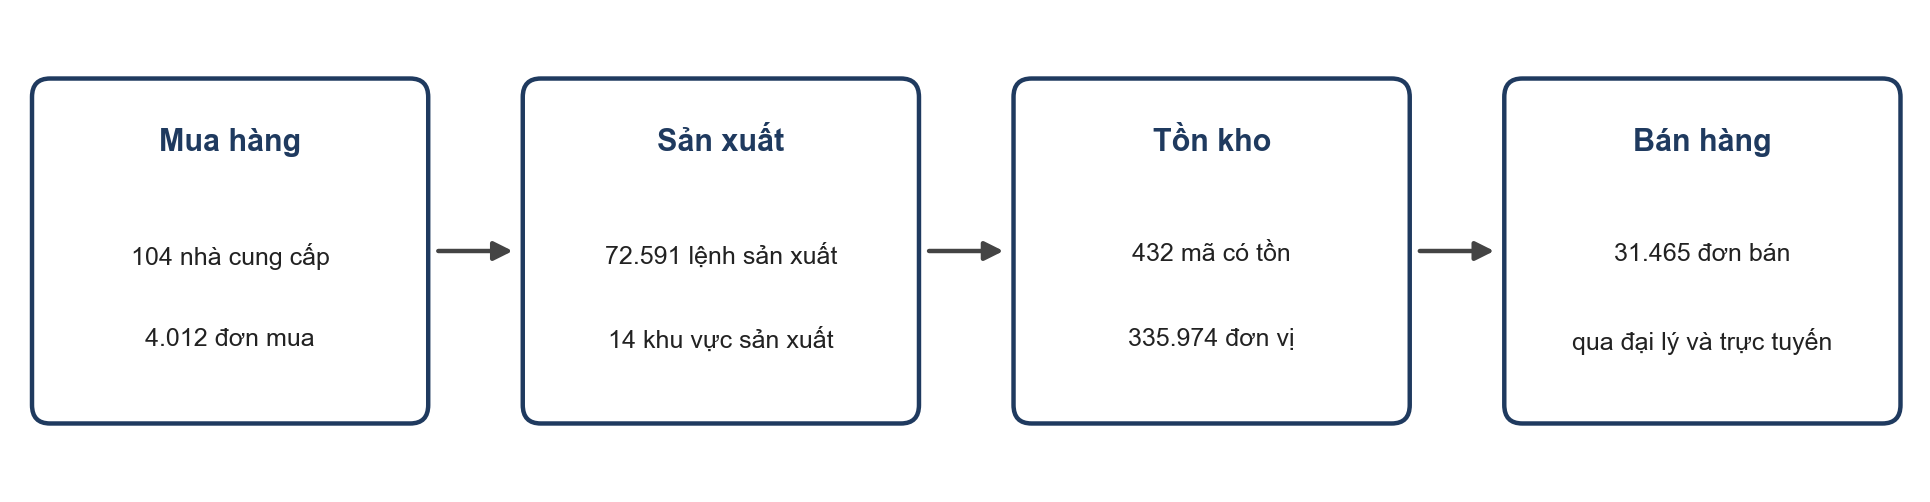
\includegraphics[width=0.95\textwidth]{chuoi_gia_tri.png}
\caption{Chuỗi hoạt động của CompanyX và quy mô từng khâu theo dữ liệu}
\label{fig:chuoi}
\end{figure}

\subsection{Mua hàng}
Công ty làm việc với 104 nhà cung cấp, tất cả đều đặt tại Mỹ. Từ 16/04/2011 đến 22/09/2014, công ty lập 4.012 đơn mua với 8.845 dòng chi tiết, tổng cộng 70,48 triệu USD. Việc mua hàng tăng rất nhanh: năm 2011 có 28 đơn (0,45 triệu USD), năm 2013 có 1.307 đơn (22,17 triệu USD), và riêng năm 2014 đã có 2.425 đơn (43,52 triệu USD). Về mức tín nhiệm (thang từ 1 đến 5), 84 trong 104 nhà cung cấp ở mức 1. Năm nhà cung cấp lớn nhất theo giá trị mua gồm Superior Bicycles (5,03 triệu USD), Professional Athletic Consultants (3,38 triệu USD), Chicago City Saddles (3,35 triệu USD), Jackson Authority (2,82 triệu USD) và Vision Cycles, Inc. (2,78 triệu USD).

\subsection{Sản xuất}
CompanyX tự sản xuất toàn bộ 97 mã xe đạp và 115 trong 134 mã linh kiện. Từ 03/06/2011 đến 02/06/2014, công ty ghi nhận 72.591 lệnh sản xuất với khoảng 4,51 triệu đơn vị, trong đó 10.651 đơn vị bị loại bỏ (phế phẩm), tương đương 0,24\%. Mỗi sản phẩm lắp ráp có danh sách nguyên liệu đi kèm: có 2.679 dòng danh sách nguyên liệu cho 238 sản phẩm lắp ráp. Công ty có 14 khu vực làm việc: bảy khu vực sản xuất có tính chi phí (tạo khung, hàn khung, mài và đánh bóng, sơn, sơn đặc biệt, lắp ráp phụ, lắp ráp hoàn chỉnh) và bảy khu vực phụ trợ như kho dụng cụ, kho kim loại, kho sơn và kho thành phẩm. Còn 432 mã tồn kho, tổng 335.974 đơn vị.

\begin{table}[H]
\centering
\small
\begin{tabular}{lrr}
\toprule
Năm & Lệnh sản xuất & Số đơn vị sản xuất \\
\midrule
2011 (từ 03/06) & 8.904 & 379.094 \\
2012 & 18.693 & 1.304.350 \\
2013 & 28.905 & 1.909.963 \\
2014 (đến 02/06) & 16.089 & 914.314 \\
\midrule
Tổng & 72.591 & 4.507.721 \\
\bottomrule
\end{tabular}
\caption{Sản xuất theo năm}
\end{table}

\section{Sản phẩm}
CompanyX có 504 mã sản phẩm, thuộc 119 mẫu sản phẩm. Các mã được chia thành bốn nhóm bán ra, cùng một nhóm chi tiết nội bộ dùng để lắp ráp (Bảng~\ref{tab:nhom}). Giá niêm yết dao động từ 2,29 USD (một phụ kiện nhỏ) đến 3.578,27 USD (xe đạp cao cấp).

\begin{table}[H]
\centering
\small
\begin{tabular}{p{4.3cm}rrp{4.6cm}}
\toprule
Nhóm & Số mã & Tự sản xuất & Giá niêm yết (USD) \\
\midrule
Xe đạp (Bikes) & 97 & 97 & 539,99 đến 3.578,27 \\
Linh kiện (Components) & 134 & 115 & 20,24 đến 1.431,50 \\
Trang phục (Clothing) & 35 & 0 & 8,99 đến 89,99 \\
Phụ kiện (Accessories) & 29 & 0 & 2,29 đến 159,00 \\
Chi tiết nội bộ, nguyên liệu & 209 & 27 & phần lớn không bán (200 mã giá 0) \\
\midrule
Tổng & 504 & 239 & \\
\bottomrule
\end{tabular}
\caption{Bốn nhóm sản phẩm bán ra và nhóm chi tiết nội bộ}
\label{tab:nhom}
\end{table}

\begin{itemize}
    \item \textbf{Xe đạp:} có ba loại là xe đường trường (Road Bikes, 43 mã), xe địa hình (Mountain Bikes, 32 mã) và xe du lịch (Touring Bikes, 22 mã). Đơn giá trung bình của các dòng bán xe khoảng 1.254 USD.
    \item \textbf{Linh kiện:} gồm khung xe (79 mã, chia cho ba loại xe), bánh xe (14), yên xe (9), tay lái (8), bàn đạp (7) và các bộ phận khác như phuộc, bộ đùi đĩa, phanh, bộ chuyển líp, xích.
    \item \textbf{Trang phục:} áo đạp xe (8 mã), quần ngắn (7), găng tay (6), tất (4), cùng quần bó, áo gile, quần yếm và mũ.
    \item \textbf{Phụ kiện:} 12 loại, nhiều nhất là lốp và săm (11 mã), rồi mũ bảo hiểm, bình nước và giá đỡ, đèn (mỗi loại 3 mã), bơm (2 mã).
\end{itemize}

Về vòng đời, các sản phẩm bắt đầu được bán từ 30/04/2008 đến 30/05/2013. Tính đến cuối dữ liệu, 98 mã đã ngừng bán và 406 mã chưa có ngày ngừng bán.

\section{Bán hàng}
\subsection{Quy mô và hai kênh bán}
CompanyX có hai kênh bán hàng với tính chất rất khác nhau.
\begin{itemize}
    \item \textbf{Kênh đại lý:} 3.806 đơn (12,1\% số đơn), do nhân viên bán hàng phụ trách, giao bằng vận tải hàng hoá. Đơn trung bình khoảng 21.131 USD tiền hàng. Kênh này mang lại 80,43 triệu USD, chiếm 73,3\% doanh thu. Dữ liệu có 701 cửa hàng đại lý, trong đó 635 tài khoản đại lý có đơn.
    \item \textbf{Kênh trực tuyến:} 27.659 đơn (87,9\%) của 18.484 khách cá nhân, giao bằng xe tải đường bộ, không qua nhân viên bán hàng. Đơn trung bình khoảng 1.061 USD, tổng 29,36 triệu USD (26,7\% doanh thu).
\end{itemize}
Nói ngắn gọn, đại lý mang lại phần lớn tiền, còn trực tuyến mang lại phần lớn số đơn và số khách. Trong tổng 31.465 đơn, có 31.150 đơn ở trạng thái đã gửi và 315 đơn ở trạng thái 6, không phải đã gửi. Công ty có 17 nhân viên bán hàng.

\begin{figure}[!htbp]
\centering
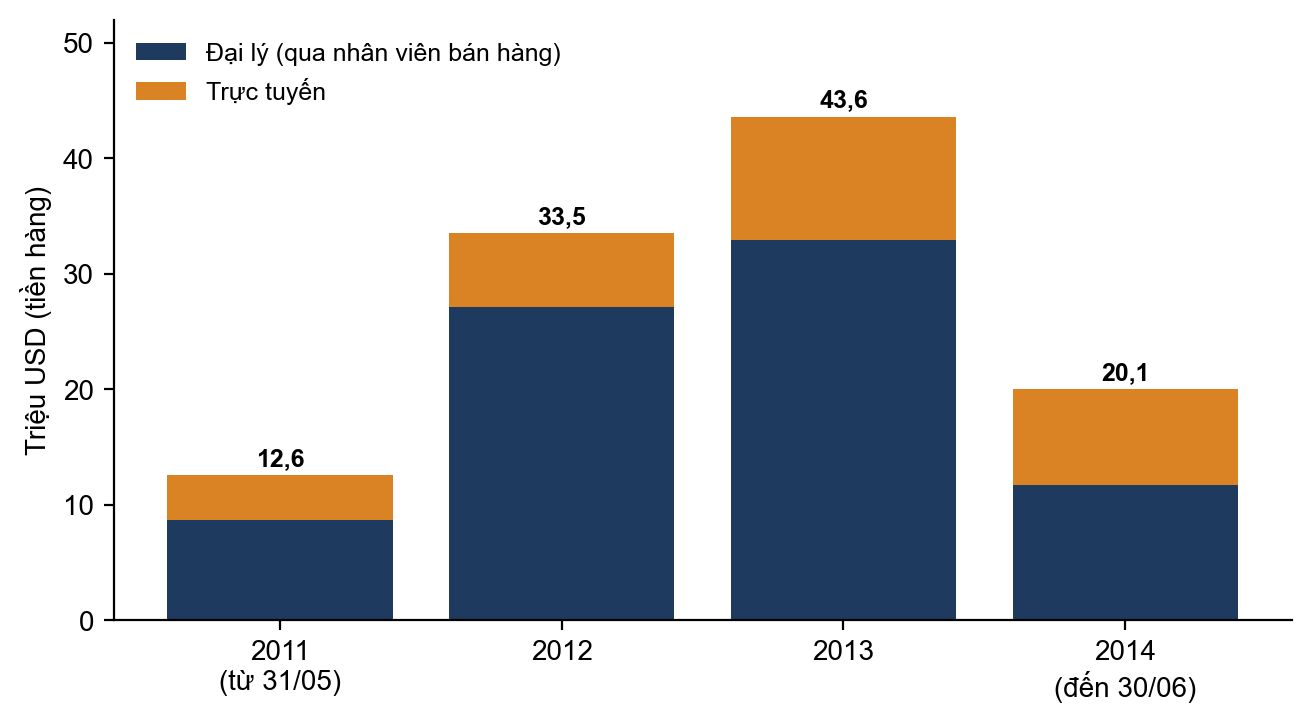
\includegraphics[width=0.6\textwidth]{doanh_thu_nam_kenh.png}
\caption{Doanh thu tiền hàng theo năm và theo kênh bán}
\label{fig:namkenh}
\end{figure}

\subsection{Tăng trưởng theo thời gian}
Số đơn tăng rất mạnh qua các năm (Hình~\ref{fig:namkenh}): 1.605 đơn trong 7 tháng cuối năm 2011, 3.917 đơn năm 2012, 14.182 đơn năm 2013 và 11.761 đơn chỉ trong nửa đầu năm 2014. Phần lớn mức tăng đến từ kênh trực tuyến, kênh này chiếm 75\% số đơn năm 2011, 70\% năm 2012, 89\% năm 2013 và 95\% năm 2014. Số khách có đơn trong năm cũng tăng từ 1.406 (2011) lên 3.162 (2012) và 11.095 (2013). Riêng doanh thu đại lý đạt đỉnh năm 2013 (32,89 triệu USD).

\subsection{Doanh thu theo nhóm hàng}
Xe đạp là nguồn doanh thu gần như duy nhất của công ty (Bảng~\ref{tab:nhomdt}, Hình~\ref{fig:nhomnam}). Linh kiện đứng thứ hai nhưng chỉ bán cho đại lý. Trang phục và phụ kiện bán được nhiều sản phẩm nhưng giá nhỏ.

\begin{table}[H]
\centering
\small
\begin{tabular}{lrrrr}
\toprule
Nhóm & Mã đã bán & Số lượng & Doanh thu (USD) & Tỷ trọng \\
\midrule
Xe đạp & 97 & 90.221 & 94.597.297 & 86,2\% \\
Linh kiện & 111 & 49.032 & 11.796.253 & 10,7\% \\
Trang phục & 34 & 73.651 & 2.119.739 & 1,9\% \\
Phụ kiện & 24 & 61.920 & 1.271.447 & 1,2\% \\
\midrule
Tổng & & 274.824 & 109.784.736 & 100\% \\
\bottomrule
\end{tabular}
\caption{Doanh thu theo nhóm hàng (thành tiền dòng chi tiết)}
\label{tab:nhomdt}
\end{table}

\begin{figure}[!htbp]
\centering
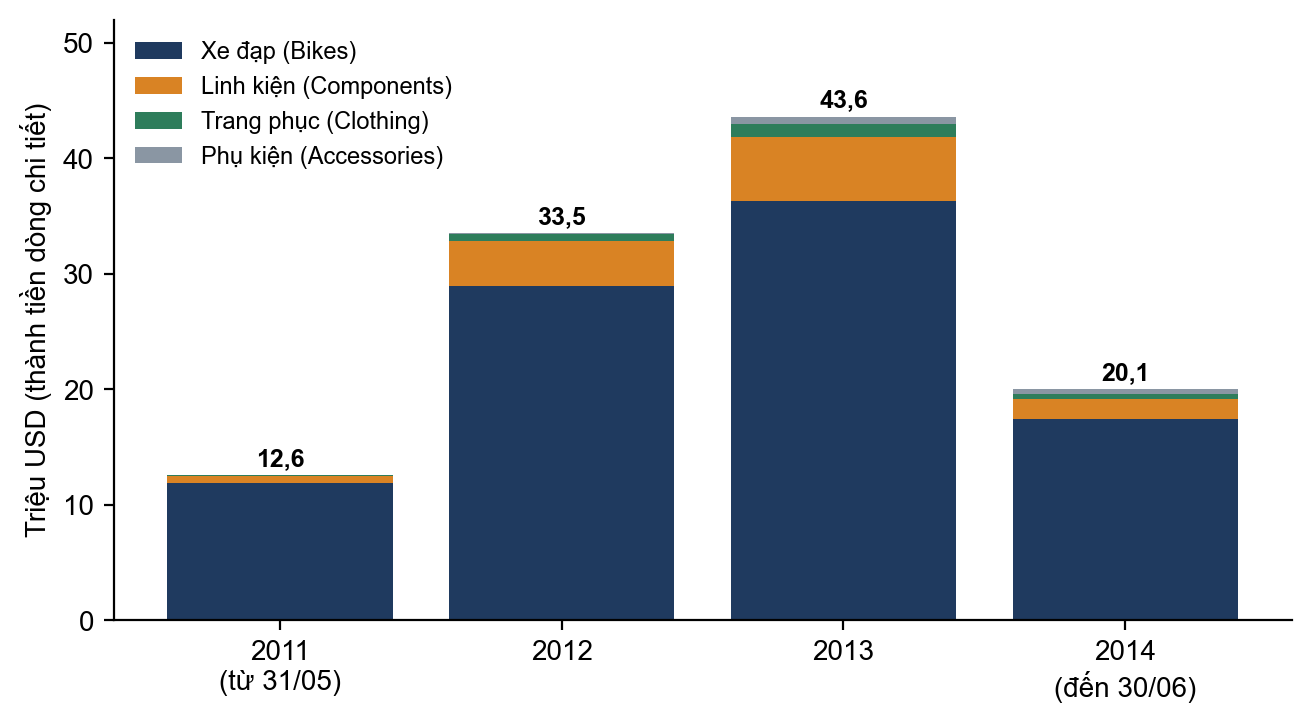
\includegraphics[width=0.6\textwidth]{doanh_thu_nhom_nam.png}
\caption{Doanh thu theo nhóm hàng và theo năm}
\label{fig:nhomnam}
\end{figure}

\textbf{Sản phẩm nổi bật.} Về doanh thu, các mẫu xe địa hình Mountain-200 dẫn đầu: mẫu Mountain-200 Black, 38 đạt 4,40 triệu USD (2.977 chiếc), kế đến là Mountain-200 Black, 42 (4,01 triệu USD) và Mountain-200 Silver, 38 (3,69 triệu USD). Về số lượng, các món rẻ lại bán nhiều nhất: mũ lưỡi trai logo (8.306 cái), bình nước 30 oz (6.815 cái), mũ bảo hiểm Sport-100 màu xanh (6.740 cái).

\subsection{Khách hàng}
Dữ liệu có 19.820 tài khoản khách, trong đó 18.484 là khách cá nhân và 1.336 gắn với cửa hàng đại lý. Có 19.119 khách phát sinh đơn. Khách cá nhân phân bố ở Bắc Mỹ (9.390 người), Châu Âu (5.503) và Thái Bình Dương (3.591). Theo phân tích của nhóm đề tài, 60,93\% khách có đơn chỉ mua đúng một lần, và với khách mua lặp lại, khoảng cách giữa hai lần mua có trung vị là 138 ngày. Đây chính là lý do công ty cần biết sớm khách nào có nguy cơ không quay lại.

\subsection{Vùng bán hàng}
CompanyX bán ở 10 vùng thuộc ba khu vực (Hình~\ref{fig:vung}). Bắc Mỹ chiếm 72,2\% doanh thu (79,29 triệu USD), Châu Âu 18,1\% (19,84 triệu USD) và Thái Bình Dương 9,7\% (10,66 triệu USD). Đại lý tập trung ở Bắc Mỹ (67,92 triệu USD), trong khi ở Châu Âu và Thái Bình Dương phần lớn doanh thu đến từ kênh trực tuyến. Riêng Australia có tới 6.843 đơn, nhiều nhất trong các vùng, nhưng gần như toàn đơn trực tuyến nhỏ nên doanh thu chỉ đứng thứ tư.

\begin{figure}[!htbp]
\centering
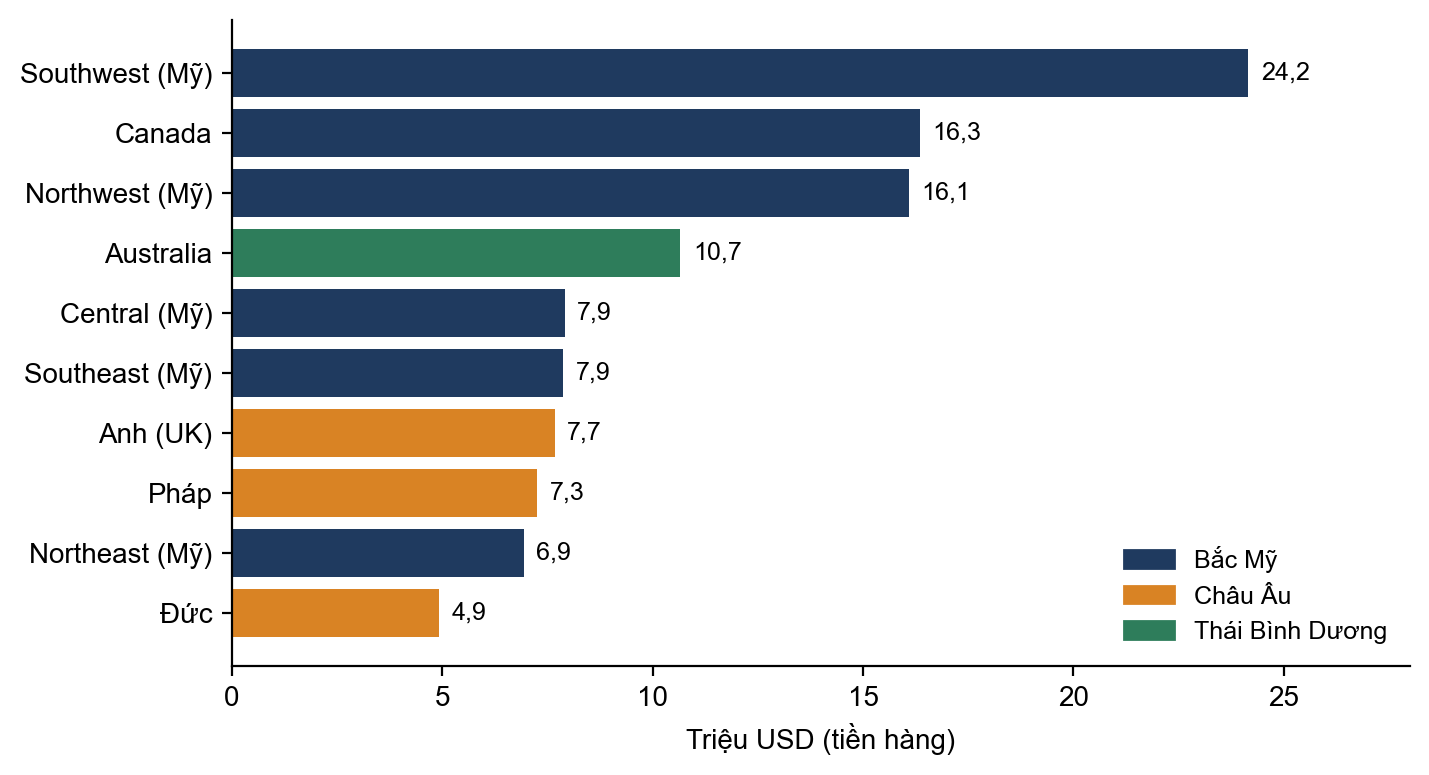
\includegraphics[width=0.6\textwidth]{doanh_thu_vung.png}
\caption{Doanh thu tiền hàng theo vùng bán hàng}
\label{fig:vung}
\end{figure}

\subsection{Khuyến mãi và giao hàng}
Công ty có 16 chương trình khuyến mãi: 5 giảm giá theo số lượng, 3 xả hàng tồn, 3 giảm giá theo mùa, 2 cho sản phẩm ngừng bán, 2 cho sản phẩm mới và 1 chương trình mặc định không giảm giá. Khuyến mãi được dùng ít: chỉ 4,48\% dòng chi tiết có áp dụng chương trình, và 3.282 dòng có chiết khấu. Về giao hàng, công ty dùng hai phương thức: xe tải đường bộ (XRQ - Truck Ground) cho đơn trực tuyến và vận tải hàng hoá (Cargo Transport 5) cho đơn đại lý.

\section{Nhân sự}
CompanyX có 290 nhân viên, 206 nam và 84 nữ, đang làm việc tại 16 phòng ban thuộc sáu khối. Phần lớn là lực lượng sản xuất: 179 người ở bộ phận Production (gồm nhiều kỹ thuật viên chia theo từng khu vực làm việc). Tiếp theo là Sales (18), Purchasing (12), Finance (10), Information Services (10) và Marketing (9). Nhân viên được tuyển từ 30/06/2006 đến 30/05/2013, và hầu hết cư trú ở bang Washington, Mỹ (275 trong 290 người, nhiều nhất ở Seattle, Bellevue, Edmonds và Redmond).

\section{Dữ liệu của CompanyX trong đề tài}
Đề tài dự đoán khách hàng rời bỏ chỉ dùng phần bán hàng trong 72 bảng của công ty, tập trung vào \textbf{18.484 khách cá nhân mua trực tuyến}. Nhóm đại lý bị loại vì họ mua theo chu kỳ nhập hàng, khác hẳn hành vi của người tiêu dùng.
\begin{itemize}
    \item \textbf{Kho dữ liệu:} dữ liệu bán hàng được tổ chức lại thành kho \texttt{CompanyX\_DW} theo mô hình hình sao (sáu bảng), chỉ giữ các đơn đã gửi của khách cá nhân.
    \item \textbf{Giới hạn của dữ liệu:} không có nhãn rời bỏ sẵn (nhóm tự định nghĩa), không có dữ liệu chăm sóc khách hàng (CRM) hay lịch sử chiến dịch, và tháng 6/2014 bất thường (930 đơn nhưng không có xe đạp nào) nên không dùng để xác định khách rời bỏ.
    \item \textbf{Kết quả của đề tài:} mô hình chấm điểm nguy cơ rời bỏ cho từng khách và một hệ hỗ trợ ra quyết định để chọn khách ưu tiên giữ chân trong ngân sách có hạn.
\end{itemize}

\section{Nguồn số liệu}
Mọi số liệu được truy vấn trực tiếp từ cơ sở dữ liệu nguồn \texttt{CompanyX} (SQL Server, chỉ đọc) ngày 05/11/2026. Doanh thu theo năm, kênh và vùng tính trên tiền hàng của cả 31.465 đơn, doanh thu theo nhóm hàng tính trên thành tiền dòng chi tiết, cả hai cho cùng tổng 109,78 triệu USD. Tỷ lệ mua một lần và khoảng cách giữa hai lần mua là kết quả phân tích của nhóm đề tài.

\end{document}
